The fruit fly, \textit{Drosophila melanogaster}, has been a great valuable tool for biological research.
Its use as a model system dates back to the beginning of the 20th century.
In 1908, Thomas H. Morgan started to grow flies in large quantities to study gene mutations. At that time, the gene concept was an abstract one, as the nature and location of the genes was still disputed.
%
The main advantages of using flies were their rapid generation time and that they were easy to culture and cheap to maintain \citep{Arias2008}.
%
In his lab at the University of Columbia, Morgan found a fly with white eyes (the wild-type eye color is red), which became a subject of his research for many years.
Eventually, he discovered that the allele of the gene, that he called \textit{white}, was located on a sex chromosome, demonstrating for the first time the sex-linkage of genes \citep{Morgan1919}.
%
Morgan's students also demonstrated that mutations were inducible with X-rays and introduced the use of "balancer" chromosomes to keep stable stocks of mutants \citep{Arias2008}.
%
%The research carried out in Morgan's lab laid the basis modern genetics, and its fly room became a central node in the genetics research, establishing \textit{Drosophila} as a organism model.

However, \textit{Drosophila}'s development was difficult to study, as the embryos were not large enough to experimentally manipulate them, and not transparent enough to visualize with a microscope \citep{Gilbert2014}.
Molecular biology techniques allowed finally to study fly genes and their effect on embryogenesis, unravelling some of the mysteries of \textit{Drosophila}'s development.
Also, histological methods (which consisted in following back to the blastoderm stage the location of larval organ precursors) and cell ablation methods (killing cells in the blastoderm and correlate its position with the position of the defects detected later) were used to create a fate map of the \textit{Drosophila} blastoderm \citep{Campos-Ortega1985} (see Fig. \ref{fig:blastoderm_fatemap} in Box 1).

In 1976, E. Lewis published a seminal work, in which he determined the effects of mutations in the Bithorax complex (BX-C).
He determined that the BX-C consisted of distinct genetic elements and that there was a correlation in the order of the mutations within the complex and the A/P order of the body affected by them \citep{Lewis1978}, a phenomenon called spatial co-linearity.
%
Lewis discoveries were complemented with the discovery of the Hox genes \citep{McGinnis1984,Scott1984}, a family of transcription factors that was shown to be conserved with vertebrates \citep{Duboule1989}.
Hox genes contain a highly conserved sequence of 180 base pairs, the homeobox, which codes for a DNA binding domain known as the homeodomain. 
%In \textit{D. melanogaster} Hox genes are arranged in two clusters, the Antennapedia (ANT-C) and the Bithorax cluster.
%But before that, Hox genes were identified as having a role in homeotic transformations.
%Homeotic transformations were first described by William Bateson \citep{Bateson1894} as a kind of natural variation found in animals, where one part of the body was transformed into another part of the body.

A milestone on the embryogenesis research on \textit{Drosophila} took place in 1980, when Eric Wieschaus and Christiane N\"{u}sslein-Volhard identified crucial genes involved in the early patterning of the \textit{Drosophila} embryo.
They systematically searched for embryonic lethal mutants, identifying 15 loci that altered the segmentation pattern of the embryo when mutated \citep{Nusslein-Volhard1980}, which they separated in tree groups based on their phenotype
%: "pattern duplication in each segment (segment polarity mutants; six loci), pattern deletion in alternating segments (pair-rule mutants; six loci) and deletion of a group of adjacent segments (gap mutants; three loci)" 
\citep{Nusslein-Volhard1980}.
%
All these genes form part of the A/P patterning cascade, whose hierarchical regulation is currently well known.

%In the next subsection, I will describe briefly the \textit{D. melanogaster} life cycle with special focus on its embryonic development.
%and the blastoderm fatemap and the relation of fate maps with gene expression maps.
%This feature, called spatial collinearity, would turn out to be a defining feature of both vertebrate and invertebrate homeotic genes. Lewis showed remarkable vision by arguing that the identity of an individual body segment is produced by the particular combination of BX-C genes, and that these were activated in reponse to an A–P gradient.
%%%%%%%%%%%%%%%%%%%%%%%%%%%%%%%%%%%%%%%%%%%%%%%%%%%%%%%%%%%%%%%%%%%%%%%%%%%%%%%%%%%%%
\label{Table_droso}
\begin{sidewaystable}
    \centering
%\begin{table}[!ht]
%\begin{adjustwidth}{-0.25in}{0in} % Comment out/remove adjustwidth environment if table fits in text column.
\caption*{\textbf{Table 1. Embryonic stages of \textit{D. melanogaster} and morphological criteria for identifying approximate ages (from \citealp{Roberts1998}) }}
\begin{tabular}{|c|p{3.5cm}|p{14cm}|}
\hline
\textbf{Stage}&\textbf{Developmental time}&\textbf{Morphologic features and main developmental events}\\
\hline
\textbf{1}	& 0 to 15min	& \textbf{Freshly laid egg.} Homogeneous cytoplasm	\\
%
\textbf{2}	& 15min to 1h 20min	&  \textbf{Early cleavage.} A cap of clear cytoplasm becomes visible at the posterior pole 	\\  
%
\textbf{3}	& 1h 20min to 1h 30min	&  \textbf{Pole cell formation.} Surface cytoplasmic layer becomes thicker and inhomogeneous	\\  
%
\textbf{4}	& 1h 30min to 2h 30min & \textbf{Syncytial blastoderm.} Nuclei divide four or more times. Cortical cytoplasm  becomes clearly delimited	from the underlaying yolk\\
%
\textbf{5}	& 2h 30min to 3h 15min	& \textbf{Cell formation.} Cell membranes move down between adjacent nuclei, separating cells	\\
%
\textbf{6}	& 3h 15min to 3h 35 min	&  \textbf{Early gastrulation.} Ventral furrow formation along the ventral midline of the embryo \\
%
\textbf{7}	& 3h 35 min to 3h 45min	&  \textbf{Midgut invaginations.} Cephaplic furrow has deepened and is visible from the side	\\
%
\textbf{8}	& 3h 45min to 4h 30min	&  \textbf{Germ band extension.} Germ band extends along the dorsal side until the posterior midgut invagination reaches the head region at 65\% length	\\
%
\textbf{9}	& 4h 30min to 5h 10min	& \textbf{Stomodeal plate formation.} Cephalic furrow no longer visible. 	 	\\
%
\textbf{10}	& 5h 10min to 6h 50min	& \textbf{Stomodeal invagination.} Anterior midgut anlage moves posteriorly. Ectodermal segmentation becomes apparent as regularly spaced	\\
%
\textbf{11}	& 6h 50min to 9h 	& \textbf{Three-layered germ band}. Segmentation is clearly visible. Due to neuroblast proliferation, the dense yolky regions gradually disappear from the head	\\
%
\textbf{12}	& 9h to 10h 30 min	& \textbf{Germ band retraction.} Yolk sac extends to the dorsal side. Anterior and posterior midgut anlagen form visible projections which gradually approach each other	\\
%
\textbf{13}	& 10h 30min to 11h 30min	& \textbf{Shortened embryo.} Germ band completely contracted. Anterior and posterior midgut have fused laterally. The head bends dorsally. Dorsal head ridge formation \\
%
\textbf{14}	& 11h 30min to 13h	& \textbf{Head involution and dorsal closure.} The germ band stretches anteriorly. Hindgut grows antero-dorsally	. Yolk sac is covered by the serosa in the dorsal middle region\\
%
\textbf{15}	& 13h to 15h 	& \textbf{Dorsal closure complete.} Subsequently constrictions divide the midgut into three regularly spaced subdivisions	\\
%
\textbf{16}	& 15h until the end of embryonic development	& \textbf{Condensation of CNS.} Conversion of the sac-like gut into a long convoluted gut. Muscular movements begin in the gut and somatic musculature. 	\\
\hline
\end{tabular}
%\end{adjustwidth}
\end{sidewaystable}
%%%%%%%%%%%%%%%%%%%%%%%%%%%%%%%%%%%%%%%%%%%%%%%%%%%%%%%%%%%%%%%%%%%%%%%%%%%%%%%%%%%%%

\subsection{\textit{D. melanogaster} life cycle}

\textit{Drosophila melanogaster} is a holometabolous insect, which means that it goes through a complete metamorphosis, i.e., the larva and the adult forms are very different. The entire life cycle is usually not longer than 10 days. Its embryonic development is very fast, the larva hatches in less than 24 hours at 25$^\circ$C. The larva grows and passes through two moults (in 4 days it increases 200-fold its weight) before becoming a resting stage called a pupa in which the body is remoulded to form the adult \citep{Stocker2008}.
Much of the adult body is formed from the imaginal discs and the abdominal histoblasts which are only present as undifferentiated buds in the larva.
%
%\subsubsection{Developmental stages}
%
%In Table 1, a brief summary of the embryonic development of \textit{D. melanogaster} is shown. For a comprehensive lecture, see \citep{Campos-Ortega1985,Roberts1998,Gilbert2014}.
%%
%The staging system shown in Table 1, correspond to the 16-stage system proposed by \citet{Roberts1998}, with approximate developmental timings at 22 $^\circ$C. 
%The numbering of the stages shown are similar to the one proposed by \citet{Campos-Ortega1985}, except that the latter add a stage 17 to the fully differentiated embryo.
%The 16-stage system is used by the BDGP \citep{Tomancak2002}. Therefore, Table 1 can serve as a reference when mentioning specific developmental stages in this work.

%\subsection{Dorso-ventral patterning}
%
%\subsection{Anterio-Posterior patterning}
%
%A milestone on the embryogenesis research on Drosophila took place in 1980, when Eric Wieschaus and Christiane N\"{u}sslein-Volhard identified crucial genes involved in the early patterning of the Drosophila embryo.
%They systematically searched for embryonic lethal mutants, identifying 15 loci that altered the segmentation pattern of the embryo when mutated \citep{Nusslein-Volhard1980}, which they separated in tree groups based on their phenotype: "pattern duplication in each
%segment (segment polarity mutants; six loci), pattern deletion in
%alternating segments (pair-rule mutants; six loci) and deletion of
%a group of adjacent segments (gap mutants; three loci)" \citep{Nusslein-Volhard1980}.
%
%All these genes form part of the A/P patterning cascade, whose hierarchical regulation is currently well known.
%
%\subsubsection{Maternal effect genes}
%The first A/P pattern of the embryo is determined in the egg chamber, during oogenesis.
%The oocyte nucleus transports \textit{Gurken} protein close to the posterior part of the egg chamber. 
%The follicle cells in that region receive the Gurken signal (Gurken is homologue of the vertebrate epidermal growth factor [EGF], see \citealp{Neuman-Silberberg1993}), which determines their fate as posterior cells.
%This signal provokes the polarization of the microtubules in an A/P axis, that facilitates the transportation of mRNAs or proteins to specific parts of the oocyte.
%Among these molecules are the mRNAs of the \textit{bicoid} and \textit{nanos}, which are transported to the anterior pole and posterior pole of the oocyte, respectively.
%These and other genes, which are known as maternal effect genes, specify the A/P axis regulating specific target genes.
%
%The maternal effect genes are classified in three different groups depending on their localization (anterior, posterior and terminal groups). Each group is briefly described below.
%
%\paragraph{Anterior group}
%After its anchorage to the anterior region of the embryo, the \textit{bicoid} mRNA is translated forming a gradient from the anterior to the posterior part of the embryo.
%This protein determines the position of the anterior structures of the embryo acting as a \textit{morphogen}, i.e., different levels of Bicoid protein determines different cell fates in the anterior part of the embryo \citep{Driever1988}.
%Bicoid is a transcription factor that regulates many target genes in a concentration-dependent manner. Foe example, expression of target genes in the head region require 1)high concentration of Bicoid and 2)the expression of \textit{hunchback}, a gene that is activated at moderate levels of Bicoid \citep{Simpson-Brose1994}.  
%
%\paragraph{Posterior group}
%The \textit{nanos} mRNA, that is localized in the posterior region of the embryo, also generates a protein gradient. Nanos inhibits the translation of \textit{hunchback} \citep{Tautz1988} by forming a complex with other ubiquitous proteins in the embryo \citep{Cho2006}. The inhibition of \textit{hunchback} by Nanos causes an anterior to posterior gradient of the former. 
%Another gene of the posterior group is the transcription factor \textit{caudal}. Contrary to \textit{nanos} or \textit{bicoid} mRNA, \textit{caudal} mRNA is distributed in the whole embryo.
%Caudal gradient is formed by translation repression by the Bicoid protein. Caudal activates genes that determine the abdominal fate. 
%The opossing gradients of Bicoid and Caudal will activate zygotic genes at different positions along the A/P axis of the blastoderm embryo.
%
%\paragraph{Terminal group}
%In mutants of terminal group genes the acron and telson are not formed \citep{Klingler1988}, which are the most anterior and posterior regions of the embryo, repectively. 
%The boundaries of these structures are defined by the Torso signal. 
%Torso is a tyrosine kinase receptor that, although is uniformly expressed along the surface membrane of early embryos, it is only activated at both poles \citep{Casanova1989}.
%
%
%
%\subsubsection{GAP gene network}
%
%Gap genes were named like that as their mutants lacked some segments in the embryo, leaving a "gap" in the embryo. 
%These genes constitute a dynamical gene network of transcription factors directly activated or repressed by the A/P gradients of the maternal effects genes.
%Their expression consist of one or two broad domains in the embryo, whose boundaries are defined by five basic regulatory mechanisms \citep{Jaeger2004}:
%%%%%%%%%%%%%%%%%%%%%%%%%%%%%%%%%%%%%%%%%%%%%%%%%%%%%%%%%%%%%%%%%%%%%%%%%%%%%%%%%%%%%%%%
%\begin{enumerate}
%\item Activation of gap genes by Bicoid and/or Caudal
%\item Auto-activation
%\item Strong repression between mutually exclusive gap genes
%\item Repression between overlapping gap genes
%\item Repression by Tolloid
%\end{enumerate}
%%%%%%%%%%%%%%%%%%%%%%%%%%%%%%%%%%%%%%%%%%%%%%%%%%%%%%%%%%%%%%%%%%%%%%%%%%%%%%%%%%%%%%%%
%
%Some of the gap genes are \textit{hunchback}, \textit{knirps}, \textit{kr\"{u}ppel} and \textit{giant}.
%Importantly, the patterning by gap gene network occurs in the late syncitial blastoderm stage, that corresponds to stage 4 and 5 in Campos-Ortega \citep{Campos-Ortega1985}.
%This allows that the nuclei, still not surrounded by membranes, regulate each other expression with transcription factors.
%
%\subsubsection{Pair-rule genes}
%
%Gap genes control then the expression of the pair-rule genes, when the embryo is still in the syncitial blastoderm stage. 
%Pair-rule genes were name like that as they are expressed in a regularly spaced striped pattern, each stripe corresponding to one parasegment.
%Parasegments, which are considered the segmental unit in the embryo, do not correspond to the segments of the larva or adult, instead, parasegments and segments are out of phase (a segment is composed by anterior and posterior compartments, a parasegment is composed by the posterior compartment of a segment and the anterior compartment of the next segment; \citealp{lawrence1992making,Arias2008}).
%%Mutants of a pair-rule genes lack the segments where the genes are normally expressed.
%
%Pair-rule genes are divided in primary and secondary pair rule genes. The former are regulated by gap and maternal effect genes, while the latter are also regulated from the primary pair
%rule genes \citep{Chipman2015}.
%The stripes of expression of pair-rule genes are modularly regulated by specific enhancers, each for one stripe or a pair of stripes.
%This was firstly discovered in the stripe 2 of the \textit{even-skipped} (\textit{eve}) gene. 
%Genetic studies determined that \textit{eve} stripe 2 is activated by Bicoid and Hunchback, while repressed by Giant and Kr\"{u}ppel \citep{Small1991,Stanojevic1991}.
%Another pair rule gene that is expressed in an alternate manner to \textit{eve} is \textit{fushi-tarazu} (\textit{ftz}).
%
%
%\subsubsection{Segment polarity genes}
%
%The next step in the A/P patterning cascade is the activation of the segment polarity genes.
%At this point blastoderm cells are already formed. Therefore, further pattern formation requires cell-cell communication \citep{Gilbert2014}.
%Segment polarity genes are regulated directly by gap and pair-rule genes and, as their name suggests, are expressed in the anterior or posterior side of the embryo para-segments.
%The genes involved in this cell to cell communication are members of the Wnt/Wingless (Wg) and Hedgehog (Hh) signalling pathways.
%
%The expression of Hh is regulated by the \textit{engrailed} gene, which in turn is activated is the cells where high levels of Even-skipped gene or Fushi Tarazu.
%Additional regulatory inputs drive the expression of \textit{engrailed} in the anterior part of each parasegment.
%Expression of \textit{wingless} is repressed by both Ftz and Eve and repressed by Odd-paired, so Wg is express only in one row of cells, adjacent to the cells expressing \textit{en}.
%A forward feedback loop \citep{Chipman2015}.
%Interaction between the Wg and Hh signaling pathways, reinforce each other expression \citep{Ingham1991,Heemskerk1991}, maintaining the pattern formed by pair-rule genes and forming a stable boundary between anterior and posterior compartments of each para-segment.
%
%\subsubsection{Hox genes}
%As mentioned before, the discovery of the Hox genes, its conservation among metazoans, and the conservation of their role in the A/P patterning, was a milestone for the emerging field of developmental genetics.
%But before that, Hox genes were identified as having a role in homeotic transformations.
%Homeotic transformations were first described by William Bateson \citep{Bateson1894} as a kind of natural variation found in animals, where one part of the body was transformed into another part of the body.
%%%%%%%%%%%%%%%%%%%%%%%%%%%%%%%%%%%%%%%%%%%%%%%%%%%%%%%%%%%%%%%%%%%%%%%%%%%%%%%%%%%%
%\begin{flushleft}
%\leftskip3em
%\rightskip\leftskip
%\footnotesize{
%\textit{
%"the case of the modification of the antenna of an insect into a foot, of the eye of a Crustacean into an antenna, of a petal into a stamen, and the like, are examples of the same kind" \citep{Bateson1894}.
%}}
%\end{flushleft}
%%%%%%%%%%%%%%%%%%%%%%%%%%%%%%%%%%%%%%%%%%%%%%%%%%%%%%%%%%%%%%%%%%%%%%%%%%%%%%%%%%%%
%
%In 1915, Calvin Bridges (who was a student of T. H. Morgan and also worked in the famous Fly room at Columbia University) isolated a spontaneous mutation in \textit{Drosophila}, in which part of the haltere (the small posterior flight appendage) was transformed into a wing tissue. Bridges called this mutant \textit{bithorax}.
%As we mentioned, it was Ed Lewis who then showed that there were several genes responsible for homeotic mutations, that these genes were arranged in two gene complexes in \textit{Drosophila}, and that the order of the genes in the chromosome correlated with the order of the segments in the A/P axis \citep{Lewis1978}.
%It was then showed that Hox genes contain a highly conserved sequence of 180 base pairs, the homeobox, which codes for a DNA binding domain known as the homeodomain. 
%Some examples of these genes are \textit{Antennapedia} (\textit{Antp}), \textit{Ultrabithorax} (\textit{Ubx}) and \textit{Abdominal-B} (\textit{Abd-B}).
%Gap genes activate and repress Hox genes, resulting in a specific expression of the latter in each of the Drosophila segments \citep{Jaeger2011}. Then, Hox genes interact between them to refine the A/P expression boundaries \citep{Hughes2002}.
%Hox genes have been said to be "selector genes" \citep{Garcia-Bellido1973,Carroll2001} as they seem to determine cell fate.

%\subsection{Fate map}

\clearpage
%%%%%%%%%%%%%%%%%%%%%%%%%%%%%%%%%%%%%%%%%%%%%%%%%%%%%%%%%%%%%%%%%%%%%%%%%%%%%%%%%%%
\begin{mdframed}[style=boxstyle,frametitle={Box1. Fate maps and gene expression maps }]
\label{Box2:Fatemap}

\paragraph{Fatemap}
The "fate map" is a very important concept in developmental biology. 
Its name refers to the practice of cartography (or map making), i.e., contructing two-dimensional (2D) representations of a usually three-dimensional (3D) space.
	\nomenclature{2D}{two-dimensional}
	\nomenclature{3D}{three-dimensional}
In a fate map the prospective fate is mapped onto the 2D representation of usually an early embryo \citep{gilbert2007fatemap}.

The first fate maps were constructed by tracking cell lineages to identify cell fate only by observation. In 1905, Conklin tracked the cell lineage of the tunicate embryo, providing the first fate map \citep{Conklin1905}. 
%In the 1930's H\"{o}rstaduius provided the fate map of the sea urchin embryo, also by cell lineage tracking. These two species were good to perform cell lineage tracking, as the number of cells of the embryo is relatively small and there are no major morphogenetic movements.
%The first method to create a fate map of the \textit{Drosophila} blastoderm were based on the analysis of gynandromorphs \citep{Janning1978}. Gynandromorphs are genetic mosaics of both male and female cells.
%Alfred H. Sturtevant analysed many gynandromorphs of \textit{Drosophila simulans} and calculated how frequently two different parts of the embryo were of the same sex. He concluded that two different parts that were more often from different sexes should come from spatially separated cleavage nuclei \citep{Janning1978}. 
%Importantly, this technique assumes that the position of a cell in the early embryo correlates with its developmental fate.
%Garcia-Bellido and Merriam improved the work of Sturtevant and using data from 379 gynandromorphs, calculated distances (in "sturt" units, in memory of Sturtevant) between the different embryo parts and construct the first fate map \citep{Garcia-Bellido1969}.
%Also, histological methods (which consisted in following back to the blastoderm the location of larval organ precursors) and cell ablation methods (killing cells in the blastoderm and correlate its position with the position of the defects detected later) were used to create a fate map of the \textit{Drosophila} blastoderm \citep{Campos-Ortega1985}.
In the 1980's Jos\'{e} A. Campos-Ortega and Volker Hartenstein combined labelling techniques (injecting horseradish peroxidase) and histological methods to create a very precise fate map of the \textit{D. melanogaster} blastoderm \citep{Campos-Ortega1985}, which is still considered a standard modern reference.
(see Figure \ref{fig:blastoderm_fatemap}).

%%%%%%%%%%%%%%%%%%%%%%%%%%%%%%%%%%%%%%%%
\par
{\centering
  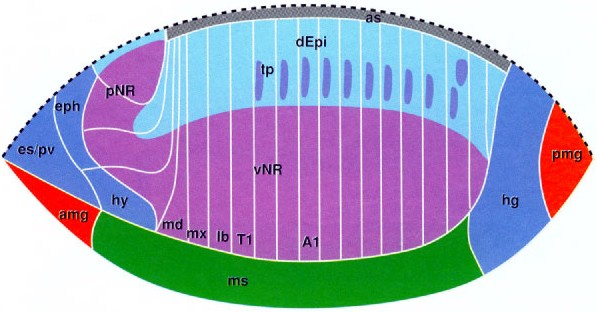
\includegraphics[width=0.45\textwidth]{./Images/blastoderm_fatemap_small.jpg}
  \centering
  \captionof{figure}{\textbf{Fate map of the \textit{Drosophila melanogaster} blastoderm}
  			The fate map is projected onto a planimetric reconstruction of the blastoderm. 
%  			The upper dashed line represents the dorsal midline and the lower margin represents the ventral midline.
  			A1 Abdominal segment 1; amg anterior midgut rudiment (endoderm); as amnioserosa; 
  			dEpi dorsal epidermis; eph epipharynx; es esophagus; hg hindgut; hy hypopharynx; 
  			lb labium; md mandible; ms mesoderm; mx maxilla;
  			pmg posterior midgut rudiment (endoderm); pNR procephalic neurogenic region; 
  			pv proventriculus; vNR ventral neurogenic region; T1 thoracic segment 1; 
  			tp tracheal placodes.
  			Diagram from \citet{Hartenstein1993}}
\label{fig:blastoderm_fatemap}
}
\par
%%%%%%%%%%%%%%%%%%%%%%%%%%%

\paragraph{Gene expression maps}

Techniques such as mRNA in situ hybridization allow to map gene expression patterns directly on the embryo, allowing the creation of "gene expression maps". In situ hybridization is based on labelled probes that are complementary to the mRNA (or DNA) that is wanted to map \citep{Gall1969}. The probe accumulates then only where the mRNA of interest is found.
Another technique to map gene expression is the use of a reporter gene. A reporter gene, which codes for a protein that can be easily identified (like the green fluorescence protein or beta-galactosidase), is linked to the regulatory region of the gene of interest so the reporter gene is going to be expressed where the gene of interest is expressed.
Gene expression maps can also be used to create (or refine) fate maps \citep{gilbert2007fatemap}. 
For example, if a gene is know to be expressed only in mesoderm precursors, mapping their gene expression in the early embryo will reveal where such mesodermal precursors are located.

%Taking advantage of recent high-throughput methods of in situ hybridization \citep{Tomancak2002,Weiszmann2009}, the expression pattern of thousands of genes through \textit{Drosophila} embryogenesis have been systematically determined \citep{Tomancak2002,Tomancak2007,Hammonds2013}, and publicly available databases have been developed \citep{Tomancak2002,Kumar2011} so any researcher can see where and when a gene is expressed in the embryo.
%These databases are suitable for computational image analysis, as the protocols used to produce the images are standardized \citep{Tomancak2002} and the images can be aligned to an anatomical view (e.g., dorsal, lateral) \citep{Kumar2011}.
%With the expression patterns of thousands of genes, gene expression maps can be made using clustering techniques, showing regions where the expression of genes is more similar.
%Frise and collaborators made such analysis, processing thousands of in situ images of the blastoderm embryo and projected them into a virtual representation of the embryo made of ca. 300 triangles \citep{Frise2010}. 
%After clustering the triangles based on their expression similarity, they produce a co-expression map that resembled the fate map shown in Figure \ref{fig:blastoderm_fatemap}.

Importantly, fate maps and gene expression maps do not necessarily have to coincide totally. Fate maps inform about which cells in the early embryo will give rise to different cell types or tissues, even when at such early stage the cells can be genetically equivalent.

\end{mdframed}
%%%%%%%%%%%%%%%%%%%%%%%%%%%%%%%%%%%%%%%%%%%%%%%%%%%%%%%%%%%%%%%%%%%%%%%%%%%%%%%%%%%
 
\subsubsection{Developmental stages}

In Table 1, a brief summary of the embryonic development of \textit{D. melanogaster} is shown. For a comprehensive lecture, see \citep{Campos-Ortega1985,Roberts1998,Gilbert2014}.
%
The staging system shown in Table 1, correspond to the 16-stage system proposed by \citet{Roberts1998}, with approximate developmental timings at 22 $^\circ$C. 
%The numbering of the stages shown are similar to the one proposed by \citet{Campos-Ortega1985}, except that the latter add a stage 17 to the fully differentiated embryo.
The 16-stage system is used by the BDGP \citep{Tomancak2002}. Therefore, Table 1 can serve as a reference when mentioning specific developmental stages in this work.

\subsection{Gene expression databases of \textit{D. melanogaster}}
\label{Intro_BDGP}

\subsubsection{Berkeley Drosophila Genome Project}
	\nomenclature{BDGP}{Berkeley Drosophila Genome Project}

The Berkeley Drosophila Genome Project (BDGP) is actually comprised of many projects, whose goals include 1) to complete the high quality sequence of the euchromatic genome of \textit{Drosophila melanogaster} and to generate and maintain biological annotations of this sequence; 2) to produce gene disruptions using P element-mediated mutagenesis; 3) to develop informatics tools that support the experimental process and identify features of DNA sequence; and 4) to characterize the sequence and spatial and temporal expression of cDNAs.

The BDGP insitu project has produced a high-throughput database of mRNA expression in different embryonic stages of \textit{D. melanogaster}, that can be used to complement and extend microarrays or RNAseq analyses \citep{Tomancak2002}. 
BDGP divides the first 16 stages of embryogenesis into six stage ranges (stages 1-3, 4-6, 7-8, 9-10, 11-12 and 13-16).

%A brief description of the hybridization protocol follows, for details see \citep{Tomancak2002}.
%For the hybridization, they used a set of cDNA clones from the Drosophila Gene Collection \citep{Stapleton2002}, to produce a digoxigenin-labeled antisense RNA probe \citep{Tomancak2002}.
%Hybridization is carried out in fixed \textit{Drosophila} embryos in 96-well plates. Successful hybridization plates are mounted on slides to document the expression pattern of each gene with high-resolution digital photographs. Then each image is assigned to one of six developmental stage ranges \citep{Weiszmann2009a}.
%
The BDGP uses high-throughput methods of in situ hybridization (for details see \citealp{Tomancak2002,Stapleton2002} to document the expression pattern of each gene with high-resolution digital photographs \citep{Weiszmann2009a}. Then, images and annotation data are stored in a modified version of Gene Ontology database. The entire dataset is available to browse or can be download from its webpage (http:// insitu.fruitfly.org/cgi-bin/ex/insitu.pl).

%Taking advantage of recent high-throughput methods of in situ hybridization \citep{Tomancak2002,Weiszmann2009}, the expression pattern of thousands of genes through \textit{Drosophila} embryogenesis have been systematically determined \citep{Tomancak2002,Tomancak2007,Hammonds2013}, and publicly available databases have been developed \citep{Tomancak2002,Kumar2011} so any researcher can see where and when a gene is expressed in the embryo.
Databases like BDGP are suitable for computational image analysis, as the protocols used to produce the images are standardized \citep{Tomancak2002} and the images can be aligned to an anatomical view (e.g., dorsal, lateral) \citep{Kumar2011}.
An example of the power of using a computational image analysis approach is the work of Frise and collaborators.
\citet{Frise2010} analysed the spatial expression pattern of 1800 genes (from the BDGP database) in the blastoderm stage of \textit{Drosophila}, projecting them onto a virtual representation of the embryo made of ca. 300 triangles.
After clustering the triangles based on their expression similarity, they produced a co-expression map that resembled the fate map shown in Figure \ref{fig:blastoderm_fatemap} (see Box 1 for a brief discussion of the relation between fate map and expression map).

%In here I used data from the BDGP insitu project whether by directly downloading data from their webpage (e.g., gene expression annotation data) or indirectly from the FlyExpress database (see next section). 

\subsubsection{Flyexpress}

The FlyExpress database (http://www.flyexpress.net/) contains a digitalized library of computationally filtered and standardized images from the high-throughput databases of mRNA expression Fly-FISH and BDGP, and from and peer-reviewed publications. It contains an image-matching search engine that can be used to search for many genes with similar or overlapping patterns of expression in the developing embryo.

The high-throughput databases from which FlyExpress extracts and computationally filter gene expression data differ in the hybridization protocol they use, the number of stages and the staging system, making direct comparisons between them difficult.
In contrast with the BDGP database (described in the previous subsection), Fly-FISH uses fluorescence in-situ hybridization probes \citep{Lecuyer2007} a 17-stage system (compared to a 16-stage system in BDGP) and five stage ranges (compared to six in BDGP).
%These databases also differ in the number of stages and the staging system, making comparisons between them difficult.
FlyExpress uses a semi-automated pipeline to standardize and align embryos, separating the multi- embryo images of BDGP into single images and discarding partial embryo images \citep{Konikoff2012}. 
After that, images are assigned to one of three anatomical views: dorsal, ventral or lateral. Therefore, the expression pattern of a gene at a specific stage and view could be represented in FlyExpress by more than one in-situ image in more than one anatomical view.


In this work, from the images available in FlyExpress, I downloaded only those from BDGP, since BDGP uses more stage ranges than FlyFISH and these represent better the whole embryogenesis of \textit{D. melanogaster}. In the Fly-FISH database is focused specially on the early stages, as the last eight developmental stages are contained in one stage range (stages 10-17).
I used the FlyExpress database, instead of the BDGP directly, because the standardization protocol used by FlyExpress produces images with embryos in the same orientation and with a cleared background that are more suitable for image computational analysis.

%In addition to the methods, these databases differ in the number of stages and the staging system, making comparisons between them difficult. We used only the images coming from BDGP, since these expand over more developmental stages than the Fly-FISH database.
